\documentclass[aspectratio=169]{beamer}

% ---------- Core packages ----------
\usetheme[numbering=fraction,progressbar=foot]{metropolis}
\metroset{sectionpage=none, subsectionpage=none}
\usepackage{amsmath,amssymb,mathtools}
\usepackage{booktabs,graphicx,microtype}
\usepackage[numbers,sort&compress]{natbib}
\bibliographystyle{abbrvnat}
\usepackage{xurl}
\urlstyle{same}
\usepackage{hyperref}

% Compact bibliography
\renewcommand{\bibsection}{}
\setlength{\bibsep}{1pt plus 0.3ex}
\setbeamertemplate{bibliography item}[text]
\makeatletter
\def\AtBeginBibliography{\footnotesize}
\makeatother

% ---------- JHU color palette ----------
\definecolor{JHUblue}{RGB}{0,45,114}
\definecolor{JHUlightblue}{RGB}{0,100,210}
\definecolor{JHUgray}{RGB}{100,100,100}

% Apply to Metropolis elements
\setbeamercolor{palette primary}{bg=JHUblue, fg=white}
\setbeamercolor{palette secondary}{bg=JHUlightblue, fg=white}
\setbeamercolor{palette tertiary}{bg=JHUblue, fg=white}
\setbeamercolor{frametitle}{fg=white,bg=JHUblue}
\setbeamercolor{title separator}{fg=JHUlightblue}
\setbeamercolor{progress bar}{fg=JHUblue,bg=gray!20}
\setbeamercolor{structure}{fg=JHUblue}
\setbeamercolor{alerted text}{fg=JHUlightblue}
\setbeamercolor{section title}{fg=white,bg=JHUblue}

\setbeamerfont{title}{series=\bfseries,size=\Large}
\setbeamerfont{frametitle}{series=\bfseries,size=\large}

\hypersetup{
  colorlinks=true,
  linkcolor=JHUblue,
  urlcolor=JHUlightblue,
  citecolor=JHUlightblue
}

% Title info
\title{Deep Reinforcement Learning for Cryptocurrency Portfolio Management}
\subtitle{Comparing Value-Based and Policy Gradient Methods}
\author{Jose Márquez Jaramillo, Taylor Hawks}
\institute{Johns Hopkins University \\ EN.605.741 Reinforcement Learning}
\date{December 2025}

\begin{document}

% ---------- Title Page ----------
{
\setcounter{framenumber}{0}
\begin{frame}[plain]
  \titlepage
\end{frame}
}

% =========================
% Slide 1: Motivation
% =========================
\begin{frame}{Motivation: Why RL for Crypto Portfolios?}
\footnotesize

\begin{columns}[T,totalwidth=\textwidth]
\begin{column}{0.55\textwidth}
\textbf{The Challenge}
\begin{itemize}\setlength{\itemsep}{2pt}
  \item Cryptocurrency markets exhibit \textbf{extreme volatility} and regime shifts
  \item Static allocation rules (equal-weight, market-cap) are suboptimal~\citep{demiguel2009optimal}
  \item Classical optimization (Mean-Variance) assumes stationarity~\citep{markowitz1952portfolio}
\end{itemize}

\vspace{0.3em}
\textbf{Why Reinforcement Learning?}
\begin{itemize}\setlength{\itemsep}{2pt}
  \item Focus on \textbf{optimal actions}, not predicting returns
  \item Natural framework for \textbf{sequential decision-making}
  \item Can learn \textbf{adaptive, cost-aware} rebalancing policies~\citep{jiang2017eIIE}
  \item No assumptions about return distributions
\end{itemize}
\end{column}

\begin{column}{0.45\textwidth}
\textbf{Research Questions}
\begin{enumerate}\setlength{\itemsep}{4pt}
  \item Can deep RL agents outperform passive baselines?
  \item How do value-based vs.\ policy gradient methods compare?
  \item What role does action space design play?
\end{enumerate}

\vspace{0.3em}
\textbf{Spoiler:} The answers are nuanced!
\end{column}
\end{columns}

\end{frame}

% =========================
% Slide 2: Contributions
% =========================
\begin{frame}{Project Contributions}
\footnotesize

\begin{columns}[T,totalwidth=\textwidth]
\begin{column}{0.5\textwidth}
\textbf{Environment Innovations}
\begin{itemize}\setlength{\itemsep}{2pt}
  \item \textbf{Variable-universe handling}: Dynamic 8--35 assets with canonical indexing (37 assets)
  \item \textbf{Regime-stratified validation}: 5 distinct market conditions
  \item \textbf{Cost-aware reward}: Transaction costs (0.1\%) in learning signal
  \item \textbf{Turnover constraints}: 30\% limit via projection/penalty
\end{itemize}

\vspace{0.2em}
\textbf{Algorithmic Contributions}
\begin{itemize}\setlength{\itemsep}{2pt}
  \item \textbf{70-action delta catalog} for discrete RL
  \item \textbf{Dirichlet policy} with GRU encoder
\end{itemize}
\end{column}

\begin{column}{0.5\textwidth}
\textbf{Empirical Contributions}
\begin{itemize}\setlength{\itemsep}{2pt}
  \item \textbf{7 agents}: 3 baselines + 4 RL methods
  \item \textbf{37 cryptocurrencies} over 7+ years
  \item \textbf{Comparative analysis}: Discrete vs.\ continuous actions
  \item \textbf{Bayesian hyperparameter search} (Optuna)
\end{itemize}

\vspace{0.2em}
\textbf{Open Source}
\begin{itemize}\setlength{\itemsep}{2pt}
  \item Full codebase with reproducible experiments
  \item Modular environment for future research
\end{itemize}
\end{column}
\end{columns}

\end{frame}

% =========================
% Slide 3a: MDP Formulation - State & Action
% =========================
\begin{frame}{MDP Formulation: State \& Action Spaces}
\small

\begin{columns}[T,totalwidth=\textwidth]
\begin{column}{0.5\textwidth}
\textbf{Formal Definition}
\[
\mathcal{M} = \langle \mathcal{S}, \mathcal{A}, P, R, \gamma \rangle
\]
\vspace{-0.3em}
\scriptsize
\begin{itemize}\setlength{\itemsep}{1pt}
  \item $\mathcal{S}$: States (market data + current holdings)
  \item $\mathcal{A}$: Actions (target portfolio weights)
  \item $P$: Transition dynamics (market evolution)
  \item $R$: Reward function (returns $-$ costs)
  \item $\gamma$: Discount factor (future reward weighting)
\end{itemize}
\small

\vspace{0.4em}
\textbf{State Space} $\mathcal{S}$
\begin{itemize}\setlength{\itemsep}{3pt}
  \item Market features: $X_t \in \mathbb{R}^{A_t \times 60 \times 4}$
  \item Previous weights: $w_{t-1} \in \Delta^{A_t}$
  \item Asset mask: $m_t \in \{0,1\}^{A_t}$
\end{itemize}
\end{column}

\begin{column}{0.5\textwidth}
\textbf{Action Space} $\mathcal{A}$
\begin{itemize}\setlength{\itemsep}{3pt}
  \item Target weights on simplex: $w_t \in \Delta^{A_t}$
  \item Long-only: $w_{t,i} \geq 0$, $\sum_i w_{t,i} = 1$
  \item Fully invested (no cash position)
\end{itemize}

\vspace{0.5em}
\textbf{Constraints}
\begin{itemize}\setlength{\itemsep}{3pt}
  \item \textbf{Turnover limit}: $\|w_t - w_{t-1}\|_1 \leq 0.30$
  \item \textbf{Max allocation}: $w_{t,i} \leq 0.35$
  \item Enforced via projection (REINFORCE) or penalty (DQN)
\end{itemize}
\end{column}
\end{columns}

\end{frame}

% =========================
% Slide 3b: MDP Formulation - Reward & Dynamics
% =========================
\begin{frame}{MDP Formulation: Reward \& Dynamics}
\small

\begin{columns}[T,totalwidth=\textwidth]
\begin{column}{0.5\textwidth}
\textbf{Reward Function} $R$
\[
r_t = \underbrace{\log(w_{t-1}^\top y_t)}_{\text{portfolio return}} - \underbrace{c\|w_t - w_{t-1}\|_1}_{\text{transaction cost}}
\]
\begin{itemize}\setlength{\itemsep}{3pt}
  \item $y_t$: price relatives (close$_t$/close$_{t-1}$)
  \item $c = 0.001$ (0.1\% transaction fee)
  \item Log-return: time-additive, geometric growth
  \item Turnover constraint is \textbf{not} in reward---enforced separately
\end{itemize}
\end{column}

\begin{column}{0.5\textwidth}
\textbf{Transition Dynamics} $P$
\begin{itemize}\setlength{\itemsep}{3pt}
  \item Market evolution is exogenous (model-free RL)
  \item Universe can change (assets enter/exit monthly)
  \item Previous weights become next state's input
\end{itemize}

\vspace{0.5em}
\textbf{Discount Factor} $\gamma$
\begin{itemize}\setlength{\itemsep}{3pt}
  \item DQN/DDQN: $\gamma = 0.93$ (via Optuna search)
  \item High $\gamma$ enables longer-horizon planning
  \item REINFORCE: $\gamma = 1.0$ (undiscounted episodic)
\end{itemize}
\end{column}
\end{columns}

\end{frame}

% =========================
% Slide 4: Environment Design
% =========================
\begin{frame}{Environment Design: Key Innovations}
\footnotesize

\begin{columns}[T,totalwidth=\textwidth]
\begin{column}{0.5\textwidth}
\textbf{Variable Universe Handling}
\begin{itemize}\setlength{\itemsep}{2pt}
  \item Universe size varies: 8--35 assets per day
  \item Assets enter/exit based on listing dates
  \item \textbf{Canonical indexing}: 37-asset superset
  \item Padding + masking for consistent NN input
\end{itemize}

\vspace{0.3em}
\textbf{Action Space Implementations}
\begin{itemize}\setlength{\itemsep}{2pt}
  \item \textbf{DQN/DDQN}: 70 discrete delta actions (adjust top-K, rotate, diversify)
  \item \textbf{REINFORCE}: Continuous Dirichlet sampling
\end{itemize}
\end{column}

\begin{column}{0.5\textwidth}
\textbf{Realistic Constraints}
\begin{itemize}\setlength{\itemsep}{2pt}
  \item \textbf{Turnover limit}: $\|w_t - w_{t-1}\|_1 \leq 0.30$
  \item \textbf{DQN/DDQN}: Penalty mode ($r = -10$)
  \item \textbf{REINFORCE}: Projection onto feasible set
\end{itemize}

\vspace{0.3em}
\textbf{Feature Engineering}
\begin{itemize}\setlength{\itemsep}{2pt}
  \item 4 features per asset: OHLC returns
  \item 60-day rolling lookback window
  \item Expanding normalization (no look-ahead)
\end{itemize}

\vspace{0.3em}
\textbf{Cost-Aware Learning}
\begin{itemize}\setlength{\itemsep}{2pt}
  \item Costs in reward $\Rightarrow$ learned implicitly
  \item Not post-hoc adjustment
\end{itemize}
\end{column}
\end{columns}

\end{frame}

% =========================
% Slide 4: Agent Architectures
% =========================
\begin{frame}{Agent Architectures: Value-Based vs.\ Policy Gradient}
\scriptsize

\begin{columns}[T,totalwidth=\textwidth]
\begin{column}{0.5\textwidth}
\textbf{Value-Based: DQN \& DDQN}~\citep{mnih2015dqn,vanHasselt2016ddqn}

\vspace{0.2em}
\textit{State Encoding:}
\begin{itemize}\setlength{\itemsep}{1pt}
  \item Canonical padding (37 positions)
  \item Flatten: 8,917 dims $\rightarrow$ 256-dim projection
\end{itemize}

\vspace{0.1em}
\textit{Q-Network:}
\begin{itemize}\setlength{\itemsep}{1pt}
  \item 3-layer MLP: 256$\rightarrow$256$\rightarrow$128$\rightarrow$70
  \item Experience replay (10K), target net (100 steps)
\end{itemize}

\vspace{0.1em}
\textit{70-Action Delta Catalog}~\citep{lucarelli2020dqlcrypto}\textit{:}
\begin{itemize}\setlength{\itemsep}{1pt}
  \item Adjust top-K by $\pm$5\%, $\pm$10\%, $\pm$15\%
  \item Rotate, diversify, concentrate, rebalance
\end{itemize}
\end{column}

\begin{column}{0.5\textwidth}
\textbf{Policy Gradient: REINFORCE}~\citep{williams1992reinforce}

\vspace{0.2em}
\textit{Policy Network:}
\begin{itemize}\setlength{\itemsep}{1pt}
  \item Canonical padding (37), no flatten---preserves sequence~\citep{jiang2016drlt}
  \item GRU processes full market as single sequence
  \item \textbf{Previous weights} input (turnover awareness)
  \item 2-layer MLP head $\rightarrow$ per-asset logits
\end{itemize}

\vspace{0.1em}
\textit{Action Sampling:}
\begin{itemize}\setlength{\itemsep}{1pt}
  \item Dirichlet: $\alpha = \text{softplus}(\text{logits}) / \tau$
  \item Temperature $\tau$: tunable exploration (non-standard)
\end{itemize}

\vspace{0.1em}
\textit{REINFORCE+Baseline:}
\begin{itemize}\setlength{\itemsep}{1pt}
  \item Shared GRU encoder with value head
  \item Advantage: $A_t = G_t - V_\phi(s_t)$
\end{itemize}
\end{column}
\end{columns}

\end{frame}

% =========================
% Slide 5: Baselines
% =========================
\begin{frame}{Baseline Strategies}
\small

\begin{columns}[T,totalwidth=\textwidth]
\begin{column}{0.33\textwidth}
\textbf{Equal Weight (EW)}~\citep{demiguel2009optimal}
\begin{itemize}\setlength{\itemsep}{3pt}
  \item $w_i = 1/N$ for all assets
  \item Naive diversification
  \item Minimal turnover
  \item Strong in volatile markets
\end{itemize}
\end{column}

\begin{column}{0.33\textwidth}
\textbf{Market Cap Weight}
\begin{itemize}\setlength{\itemsep}{3pt}
  \item $w_i \propto \text{MarketCap}_i$
  \item Tracks market portfolio
  \item BTC/ETH dominated
  \item Low turnover
\end{itemize}
\end{column}

\begin{column}{0.33\textwidth}
\textbf{Mean-Variance (MVO)}~\citep{markowitz1952portfolio}
\begin{itemize}\setlength{\itemsep}{3pt}
  \item Rolling 60-day window
  \item $\max_w \, \mu^\top w - \frac{\lambda}{2} w^\top \Sigma w$
  \item Ledoit-Wolf shrinkage~\citep{ledoit2004honey}
  \item Exploits momentum
\end{itemize}
\end{column}
\end{columns}

\vspace{1em}
\centering
\footnotesize
All baselines use the same environment with identical transaction costs (0.1\%) and constraints.

\end{frame}

% =========================
% Slide 6: Experimental Setup
% =========================
\begin{frame}{Experimental Setup}
\small

\begin{columns}[T,totalwidth=\textwidth]
\begin{column}{0.5\textwidth}
\textbf{Dataset}
\begin{itemize}\setlength{\itemsep}{3pt}
  \item \textbf{Source}: CoinGecko API\\{\scriptsize\url{coingecko.com/en/api}}
  \item \textbf{Assets}: 37 cryptocurrencies
  \item \textbf{Features}: Daily OHLCV (4 features)
  \item \textbf{Period}: July 2018 -- October 2025
\end{itemize}

\vspace{0.3em}
\textbf{Temporal Splits}
\begin{table}[h]
\footnotesize
\begin{tabular}{lll}
\toprule
\textbf{Split} & \textbf{Period} & \textbf{Days} \\
\midrule
Warmup & 2018-07 -- 2018-08 & 62 \\
Train & 2018-09 -- 2023-06 & 1,848 \\
Validation & 5 regime windows & $\sim$100 \\
Test & 2024-01 -- 2025-10 & 646 \\
\bottomrule
\end{tabular}
\end{table}
\end{column}

\begin{column}{0.5\textwidth}
\textbf{Regime-Diverse Validation}~\citep{jiang2017eIIE}
\begin{itemize}\setlength{\itemsep}{2pt}
  \item 2018 Crypto Winter
  \item March 2020 COVID Crash
  \item 2021 Bull Market
  \item 2022 Deleveraging
  \item 2023 Consolidation
\end{itemize}

\vspace{0.3em}
\textbf{Hyperparameter Search}
\begin{itemize}\setlength{\itemsep}{2pt}
  \item Optuna with TPE sampler
  \item 50 trials per agent
  \item Early stopping + Q-value explosion detection
  \item Objective: Mean validation return
\end{itemize}
\end{column}
\end{columns}

\end{frame}

% =========================
% Slide 7: Main Results Table
% =========================
\begin{frame}{Results: Performance Summary}

\begin{columns}[T]
\begin{column}{0.55\textwidth}
\centering
\scriptsize
\begin{tabular}{@{}lccccc@{}}
\toprule
\textbf{Agent} & \textbf{Ret.} & \textbf{Sharpe} & \textbf{Sortino} & \textbf{MDD} & \textbf{Turn.} \\
 & \textbf{(\%)} & & & \textbf{(\%)} & \textbf{(\%)} \\
\midrule
\multicolumn{6}{l}{\textit{Baselines}} \\
Equal Weight     & 168.5 & 1.22 & 1.25 & 48.9 & \textbf{0.3} \\
Market Cap       & 159.3 & 1.24 & 1.30 & \underline{44.2} & 0.3 \\
Mean-Variance    & \textbf{366.5} & \textbf{1.64} & \textbf{1.69} & \textbf{40.0} & 13.5 \\
\midrule
\multicolumn{6}{l}{\textit{RL Agents}} \\
DQN              & 135.1 & 1.09 & 1.11 & 49.0 & 5.7 \\
DDQN             & \underline{190.8} & \underline{1.25} & \underline{1.30} & 49.9 & 6.3 \\
REINFORCE        & 161.8 & 1.20 & 1.22 & 48.8 & 0.9 \\
REINFORCE+BL     & 167.4 & 1.20 & 1.24 & 49.3 & \underline{0.4} \\
\bottomrule
\end{tabular}

\vspace{0.3em}
\tiny
Test period: Jan 2024 -- Oct 2025 (646 days)\\
Best in \textbf{bold}, second-best \underline{underlined}
\end{column}

\hfill

\begin{column}{0.42\textwidth}
\textbf{Key Findings}
\small
\begin{itemize}\setlength{\itemsep}{8pt}
  \item \textbf{MVO dominates}: 366\% return, 1.64 Sharpe ratio
  \item \alert{DDQN beats passive baselines}: 190.8\% vs.\ 168.5\% (EW)
  \item \textbf{REINFORCE competitive}: 167\% (w/ baseline) $\approx$ Equal Weight
  \item \textbf{Risk similar}: All agents experience $\sim$50\% max drawdown
\end{itemize}
\end{column}
\end{columns}

\end{frame}

% =========================
% Slide 8: Cumulative Returns Figure
% =========================
\begin{frame}{Results: Cumulative Returns \& Drawdown}

\begin{columns}[T,totalwidth=\textwidth]
\begin{column}{0.72\textwidth}
\begin{figure}
\centering
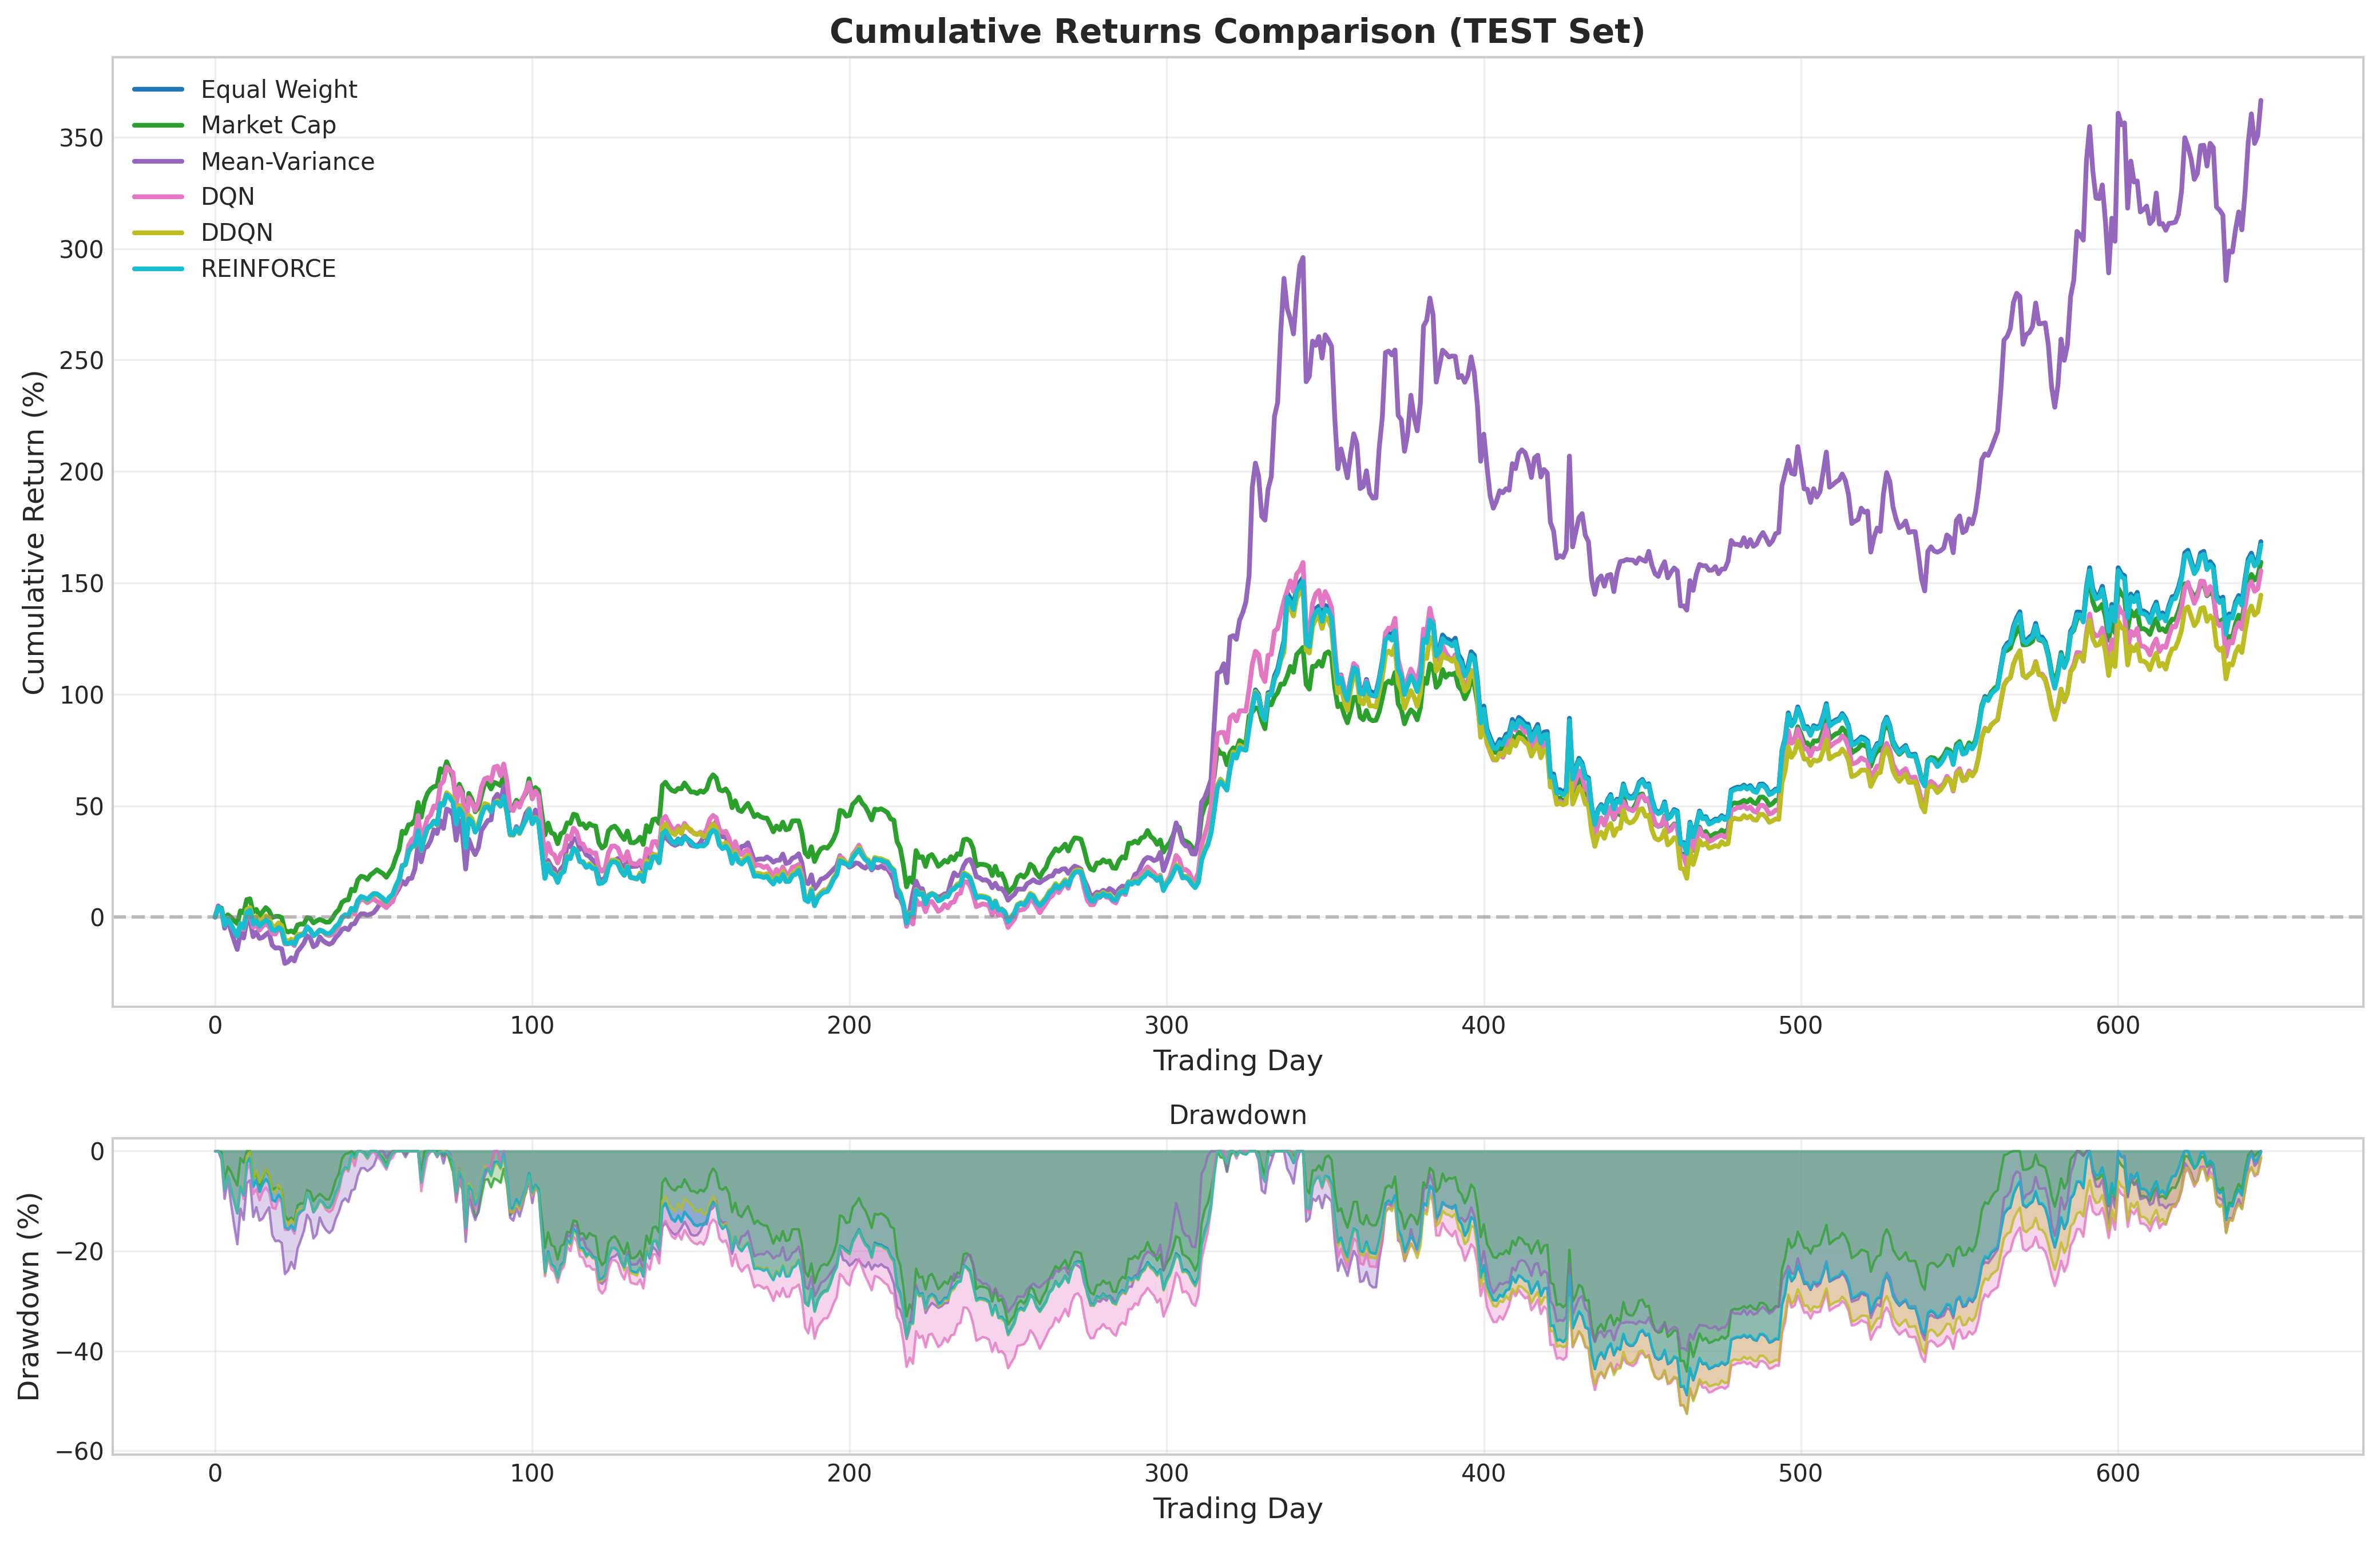
\includegraphics[width=\textwidth,height=0.82\textheight,keepaspectratio]{figures/cumulative_returns.png}
\end{figure}
\end{column}

\begin{column}{0.28\textwidth}
\small
\textbf{Observations}
\begin{itemize}\setlength{\itemsep}{5pt}
  \item MVO (red) leads throughout the period
  \item DDQN (magenta) outperforms passive baselines
  \item All agents hit $\sim$50\% drawdown mid-2024
  \item Strong recovery in late 2024
  \item REINFORCE tracks EW closely
\end{itemize}
\end{column}
\end{columns}

\end{frame}

% =========================
% Slide 9: Rolling Sharpe
% =========================
\begin{frame}{Results: Rolling Risk-Adjusted Performance}

\begin{figure}
\centering
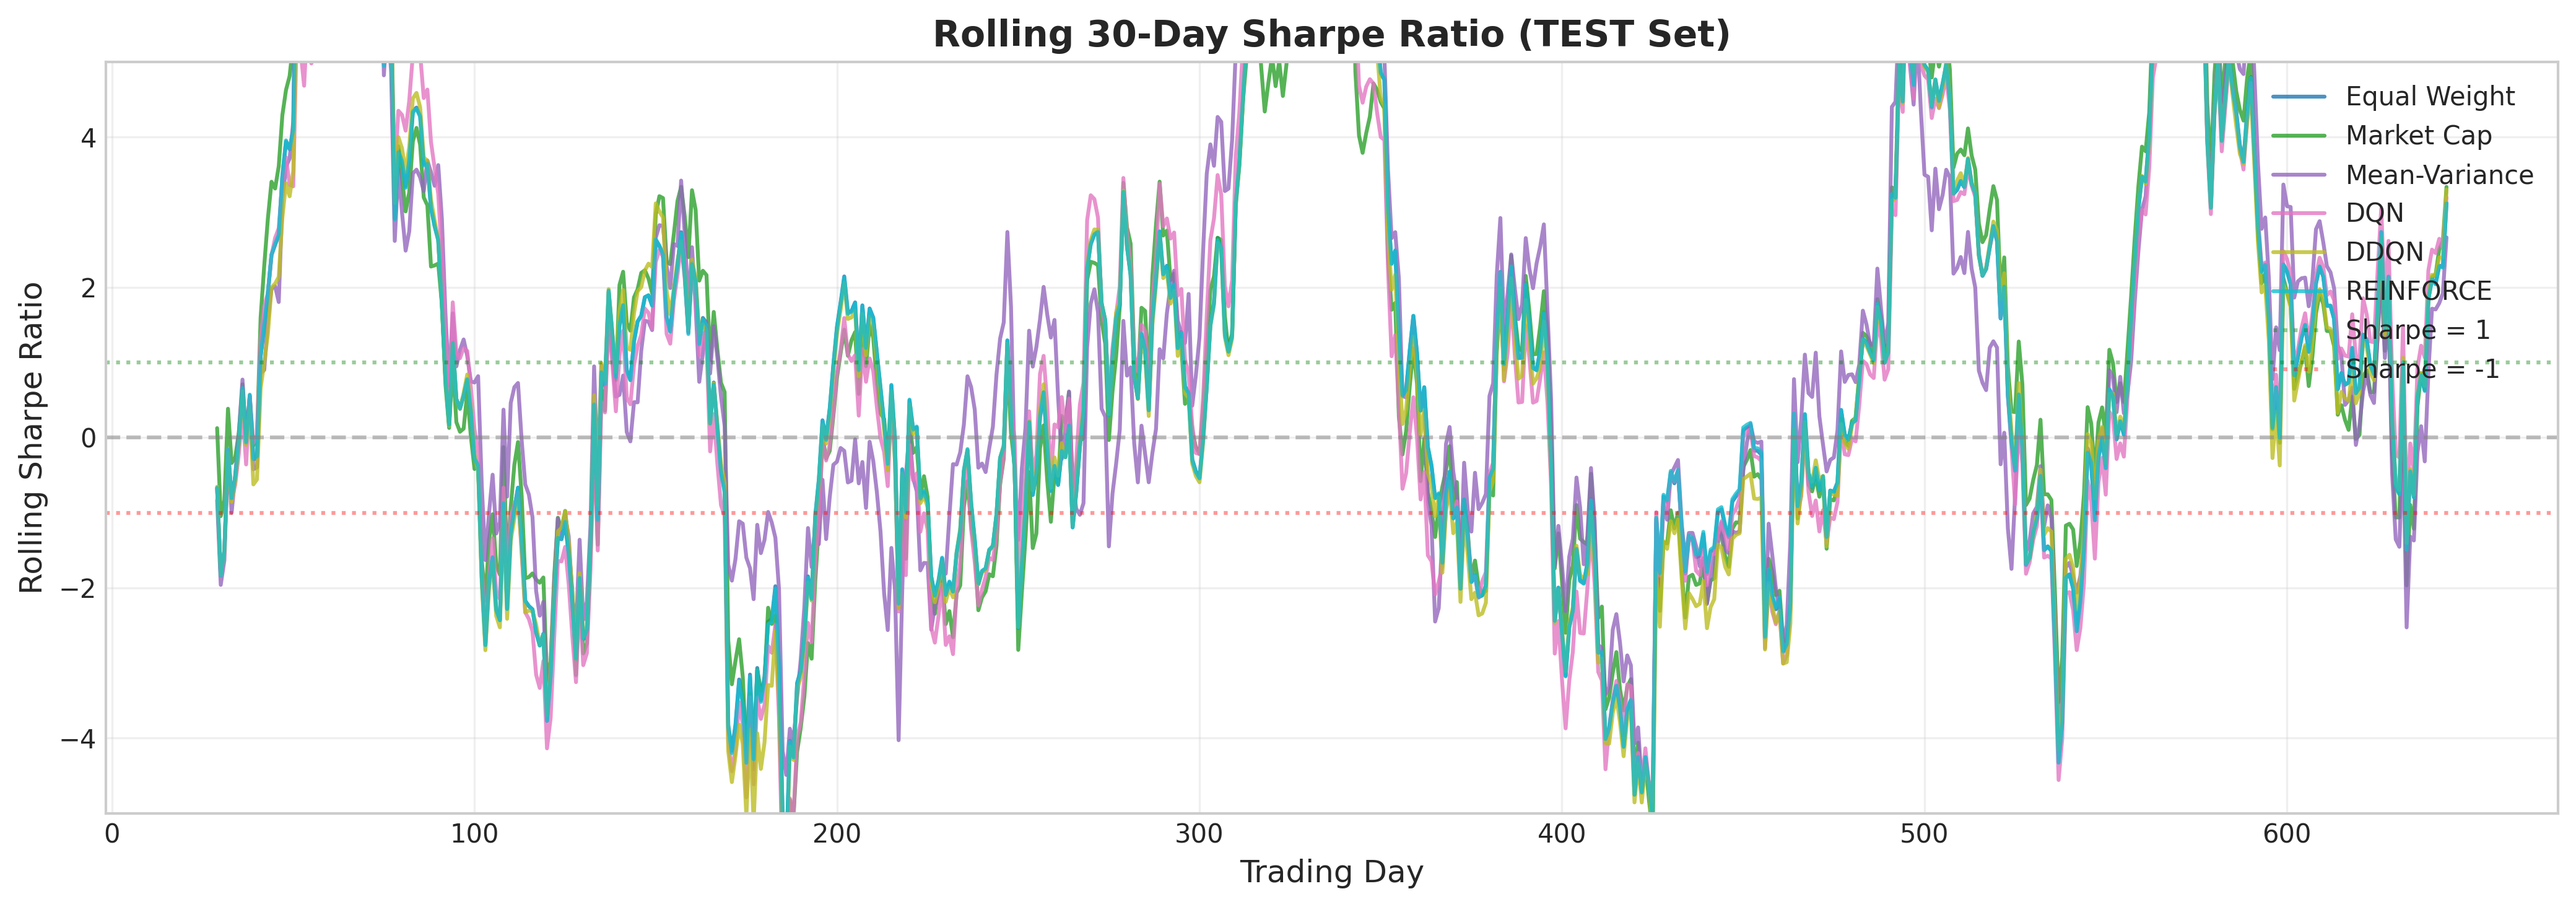
\includegraphics[width=0.92\textwidth,height=0.72\textheight,keepaspectratio]{figures/rolling_sharpe.png}
\end{figure}

\vspace{-0.3em}
\scriptsize
MVO maintains highest Sharpe. DDQN and REINFORCE competitive with passive baselines.

\end{frame}

% =========================
% Slide 10: Allocation Comparison
% =========================
\begin{frame}{Results: Portfolio Allocation Dynamics}

\begin{figure}
\centering
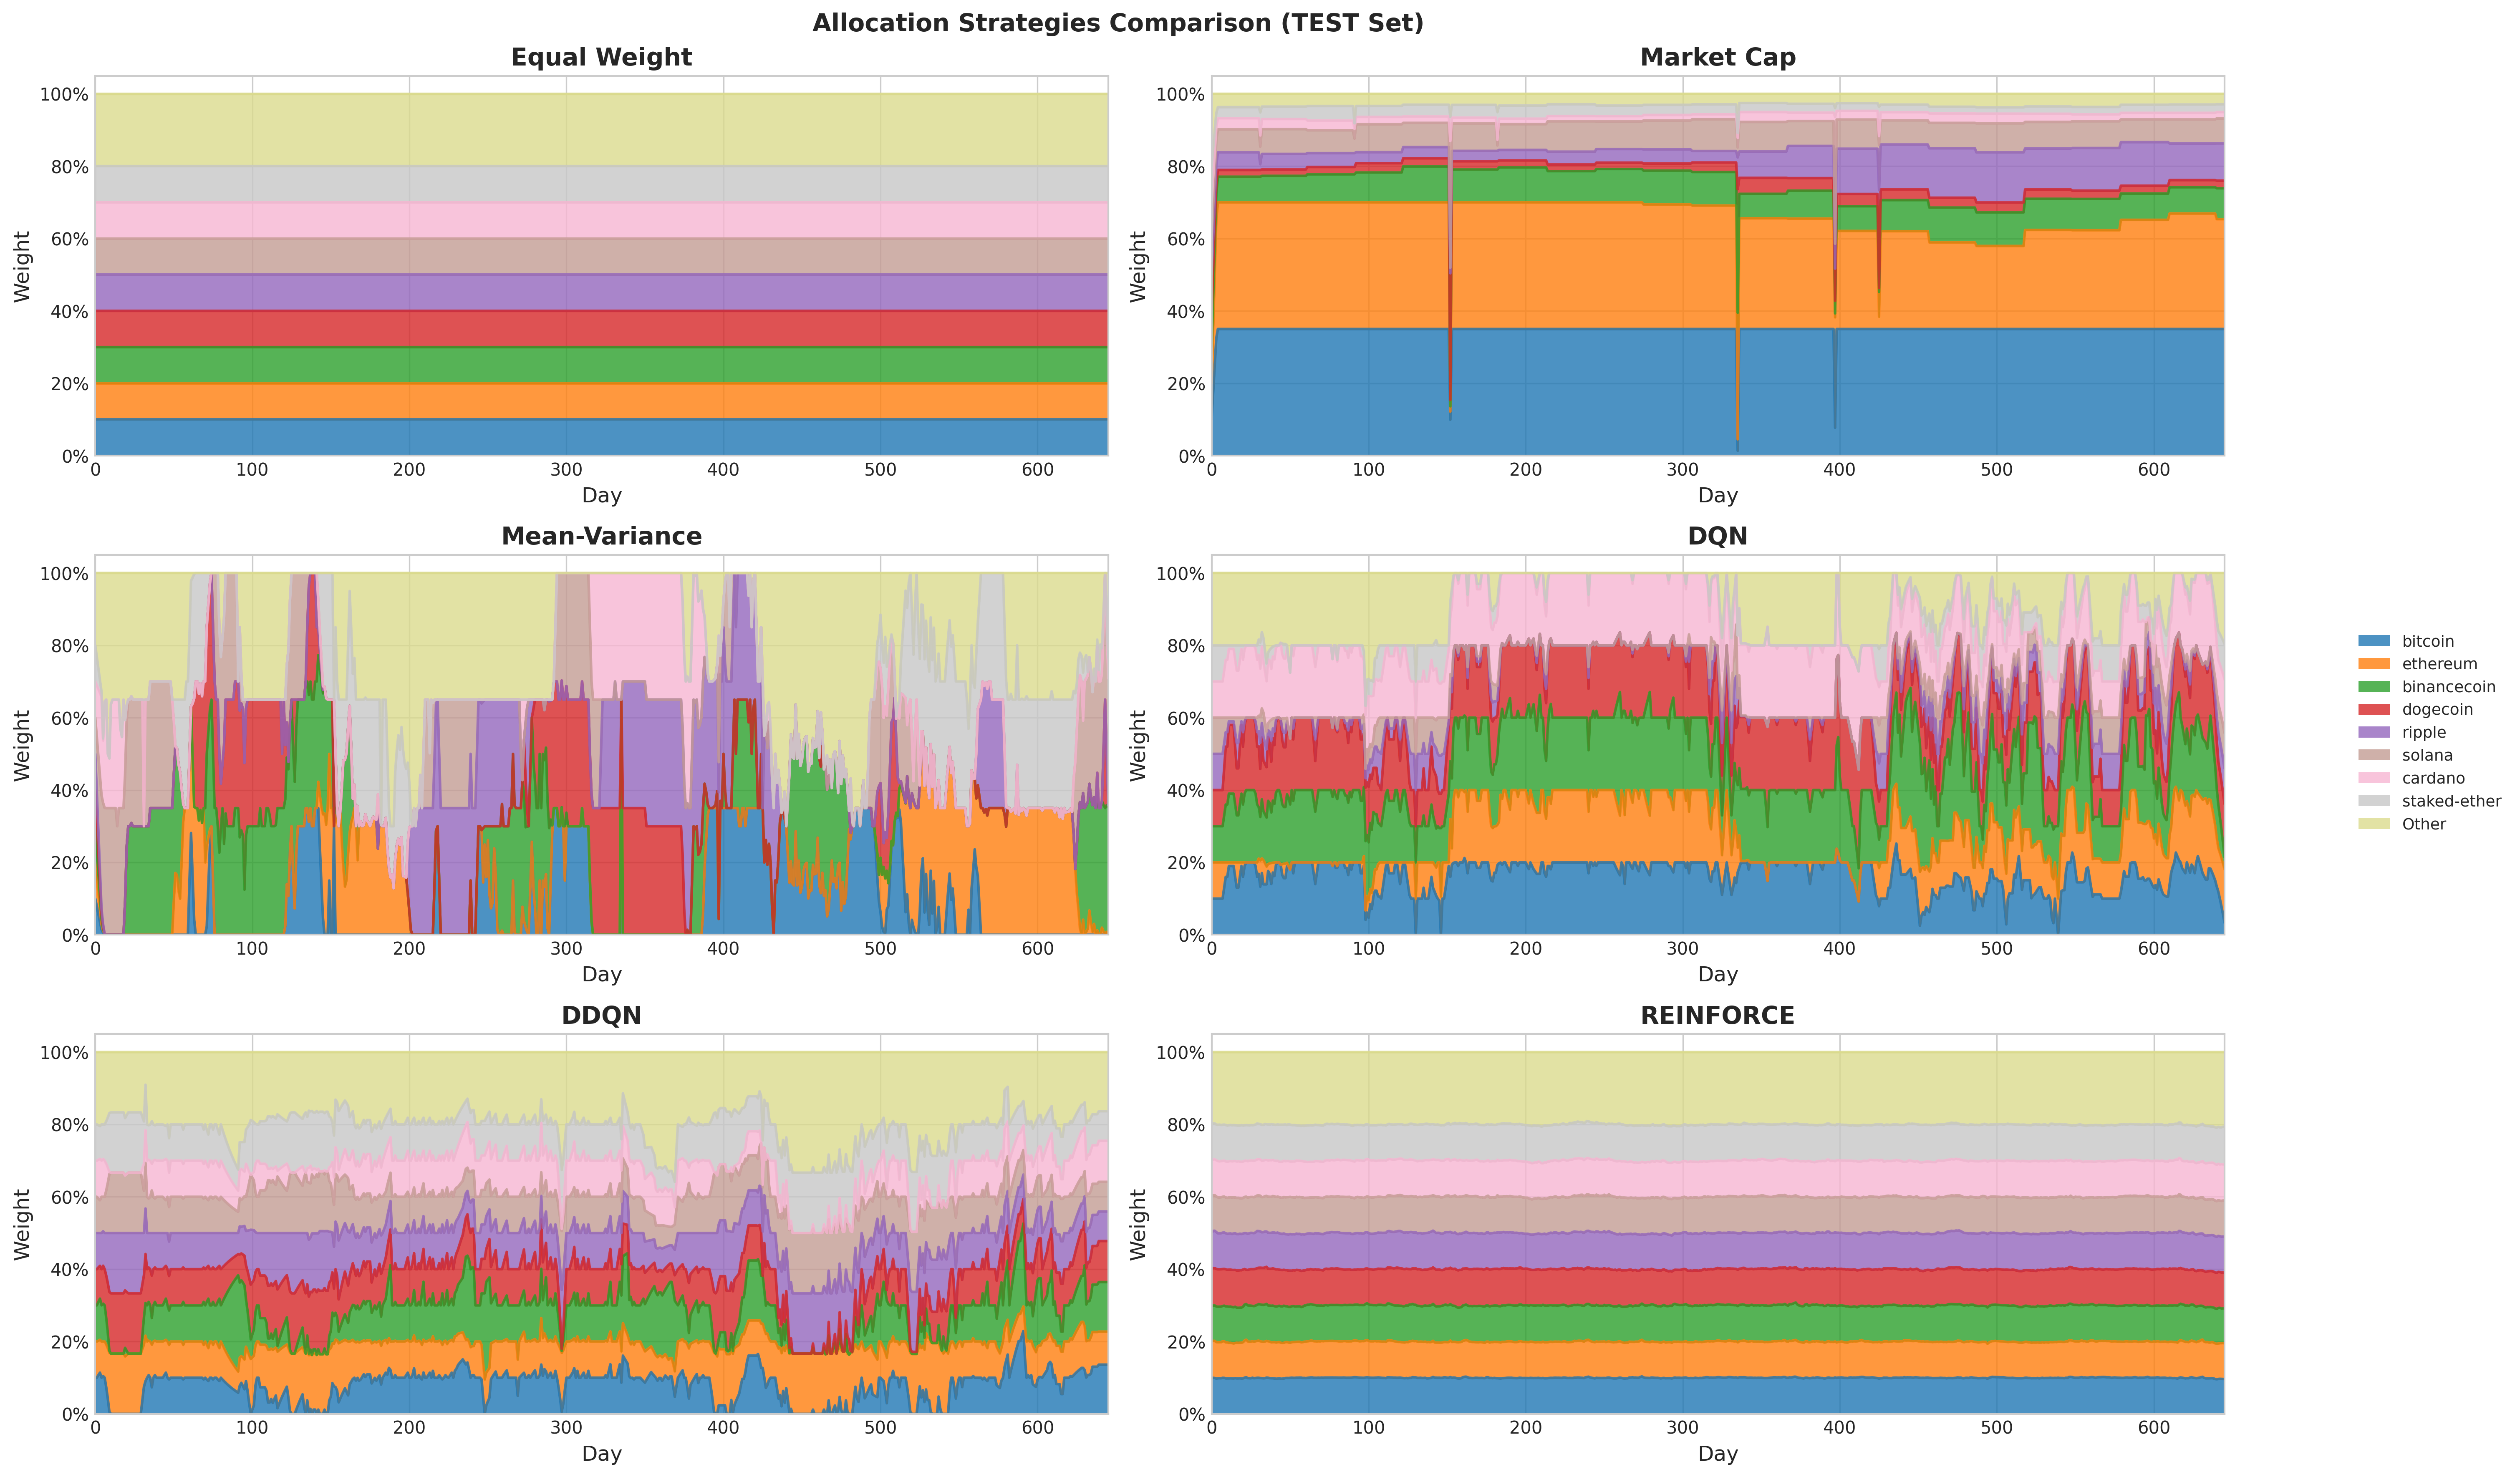
\includegraphics[width=0.98\textwidth,height=0.78\textheight,keepaspectratio]{figures/allocation_comparison.png}
\end{figure}

\vspace{-0.3em}
\scriptsize
EW: stable. Market Cap: BTC/ETH dominated. MVO/DDQN: active rebalancing. REINFORCE: stable allocations under deterministic eval.

\end{frame}

% =========================
% Slide 11: Analysis - DDQN vs REINFORCE
% =========================
\begin{frame}{Analysis: DDQN vs.\ REINFORCE Design Tradeoffs}
\small

\begin{columns}[T,totalwidth=\textwidth]
\begin{column}{0.5\textwidth}
\textbf{DDQN Success Factors}
\begin{itemize}\setlength{\itemsep}{4pt}
  \item \textbf{Delta-based actions}: Incremental adjustments with built-in turnover control~\citep{lucarelli2020dqlcrypto}
  \item \textbf{Penalty mode}: Explicit $-10$ reward for constraint violations---clear learning signal
  \item \textbf{Double Q-learning}: Reduces overestimation bias~\citep{vanHasselt2016ddqn}
  \item \textbf{Discrete choices}: Easier credit assignment
\end{itemize}

\vspace{0.3em}
\textit{Key insight:} Action space \& environment design aligned well for DQN.
\end{column}

\begin{column}{0.5\textwidth}
\textbf{REINFORCE Design Considerations}
\begin{itemize}\setlength{\itemsep}{4pt}
  \item \textbf{No programmed constraints}: REINFORCE has zero hard constraints; any constraint-like behaviour must be learned via environment feedback
  \item \textbf{Continuous outputs}: Unconstrained Dirichlet sampling can propose large jumps
  \item \textbf{Deterministic eval} resolves this: mean $\alpha_i/\sum_j\alpha_j$ produces smooth weights
  \item \textbf{Baseline helped validation, no longer hurt test}: Fixed action selection/sampling bug removed test-time penalty
\end{itemize}

\vspace{0.3em}
\textit{Lesson:} Environment design appropriate for DQN may not suit policy gradient. Output constraints on policy would have helped.
\end{column}
\end{columns}

\end{frame}

% =========================
% Slide 12: MVO Dominance
% =========================
\begin{frame}{Analysis: Why Mean-Variance Dominated}
\small

\begin{columns}[T,totalwidth=\textwidth]
\begin{column}{0.5\textwidth}
\textbf{MVO Advantages}
\begin{itemize}\setlength{\itemsep}{4pt}
  \item \textbf{Sample efficient}: Directly estimates $\mu$, $\Sigma$ from data
  \item \textbf{Closed-form solution}: No gradient descent needed
  \item \textbf{Momentum capture}: Rolling estimates naturally exploit trends
  \item \textbf{Bull market alignment}: Test period favored momentum strategies
\end{itemize}
\end{column}

\begin{column}{0.5\textwidth}
\textbf{Caveats}
\begin{itemize}\setlength{\itemsep}{4pt}
  \item \textbf{Regime-dependent}: May fail in mean-reverting or crash periods
  \item \textbf{Stationarity assumption}: Violated in crypto markets
  \item \textbf{No adaptation}: Fixed 60-day lookback
  \item \textbf{Higher turnover} (13.5\%): More sensitive to estimation noise
\end{itemize}

\vspace{0.5em}
\textit{Takeaway:} Classical methods remain formidable when conditions align!
\end{column}
\end{columns}

\end{frame}

% =========================
% Slide 13: Limitations
% =========================
\begin{frame}{Limitations}
\footnotesize

\begin{columns}[T,totalwidth=\textwidth]
\begin{column}{0.5\textwidth}
\textbf{Experimental Limitations}
\begin{itemize}\setlength{\itemsep}{3pt}
  \item \textbf{Single test regime}: Bull market (2024--2025)
  \item \textbf{Simplified costs}: No slippage or market impact
  \item \textbf{Frozen agents}: No online adaptation post-training
  \item \textbf{Search budget}: 50 trials may miss optimal configs
\end{itemize}
\end{column}

\begin{column}{0.5\textwidth}
\textbf{Design Limitations}
\begin{itemize}\setlength{\itemsep}{3pt}
  \item \textbf{Deterministic eval}: Stochastic deployment may differ
  \item \textbf{Baseline gap}: Better on validation, narrower on test
  \item \textbf{No cash position}: Fully invested at all times
  \item \textbf{Daily rebalancing}: Weekly might reduce costs
  \item \textbf{Single random seed}: For final training runs
\end{itemize}
\end{column}
\end{columns}

\vspace{0.5em}
\centering
\scriptsize
Results should be interpreted as indicative rather than definitive. Multi-regime testing essential for deployment.

\end{frame}

% =========================
% Slide 14: Conclusions & Future Work
% =========================
\begin{frame}{Conclusions \& Future Directions}
\small

\begin{columns}[T,totalwidth=\textwidth]
\begin{column}{0.5\textwidth}
\textbf{Key Takeaways}
\begin{enumerate}\setlength{\itemsep}{5pt}
  \item \textbf{DDQN beats passive baselines} (190.77\% vs.\ 168.50\%)
  \item \textbf{REINFORCE competitive} with deterministic eval (167\%)
  \item \textbf{Classical methods remain strong}: MVO achieved 366\%
  \item \textbf{Inference behavior matters}: Dirichlet mean vs.\ sampling
\end{enumerate}
\end{column}

\begin{column}{0.5\textwidth}
\textbf{Future Directions}
\begin{itemize}\setlength{\itemsep}{4pt}
  \item \textbf{Deterministic policies}: DDPG, TD3 as natural middle ground
  \item \textbf{Transformers}: Cross-asset attention for correlation modeling
  \item \textbf{Online learning}: Continuous adaptation to market regimes
  \item \textbf{Multi-regime testing}: Bear markets, crashes, consolidation
  \item \textbf{Stochastic deployment}: Study sampling vs.\ mean tradeoffs
\end{itemize}
\end{column}
\end{columns}

\vspace{0.5em}
\centering
\textbf{Code available at:} \url{https://github.com/josemarquezjaramillo/crypto-rl-portfolio}

\end{frame}

% =========================
% Slide 15: Questions
% =========================
\begin{frame}[standout]
Questions?
\end{frame}

% =========================
% References
% =========================
\begin{frame}[allowframebreaks]{References}
\footnotesize
\bibliography{bibliography}
\end{frame}

\end{document}
